\documentclass[prodmode,acmtecs]{acmsmall} \usepackage[ruled]{algorithm2e}
\usepackage{graphicx}

\acmYear{2015}
\acmMonth{4}

\begin{document}
\title{Accelerating Automated Extraction of Radio Astronomical Sources from Overseation Data with GPU Accelerators
\author{YASEEN HAMDULAY, JARRED DE BEER}
\affil {University of Cape Town}
}

\maketitle{}

\section{Project Description}


Radio astronomy surveys are blind surveys of the sky for detecting neutral hydrogen emission from galaxies. The process of detection is known as source finding and has traditionally been conducted by Astrophysicists who manually inspect the resulting data to identify sources of hydrogen emissions.


Future radio astronomy surveys, such as MeerKAT (Meer Karoo Array Telescope) and ASKAP (Australian Square Kilometer Array Pathfinder), are going to be orders of magnitude larger than traditional surveys and manual inspection of the data will no longer be viable. Automating the source finding process has become a necessity and various software packages have been developed to integrate this process. However, they are still too slow and research into accelerating them has revealed key
bottlenecks in their performance. In this project we identify algorithms from two such bottlenecks and attempt to accelerate them with CUDA (Compute Unified Device Architecture), a parallel programming model integrated into the GPUs (Graphics Processing Unit) of a range of NVIDIA graphics cards.


The GPU is a highly parallel, low-cost computational alternative to the CPU with a considerably lower energy footprint. A GPU is comprised of streaming multiprocessors which each contain dedicated arithmetic units and a variety of memory hierarchies. They exploit data level parallelism by implementing SIMD (Single Instruction Multiple Data) and MIMD (Multiple Instruction Multiple Data) performed by blocks of threads. Threads are lightweight and designed to incur minimal time penalties for
context switching, which helps maximise thread occupancy.\cite{fluke2011astrophysical} Fluke et al report that in particular cases GPU implementations of single-threaded CPU algorithms perform ten to a hundred times faster. The most performant solutions, however, can be particularly difficult to achieve due to the unique nature of GPU programming.


The algorithms we have identified as bottlenecks are the 2D-1D wavelet reconstruction and the S+C (Source and Clip) source finder. 2D-1D wavelet reconstruction is a smoothing process to remove noise from data, prior to source detection. This smoothing process is depended upon by intensity threshold source finding algorithms and consumes up to 75% of the overall runtime. The S+C source finding algorithm is an intensity threshold source finder which performs a smooth and clip operation to
detect sources and is one of two source finders integrated into the SoFiA package. SoFiA is a source finding package which is designed to be flexible and used in various types of surveys at ASKAP. In addition to implementing S+C, SoFiA has also integrated the 2D-1D wavelet reconstruction algorithm into the filtering stage of its pipeline. The package is designed to be modular which allows algorithms to be integrated by the community to further enhance its use as a general source finder
package. SoFiA is released under the GPLv2 license and is available on Github. The 2D-1D wavelet reconstruction algorithm is also used in the filtering process of the DUCHAMP package. DUCHAMP is an intensity based source finder which has the highest reliability among a range of source finders. The DUCHAMP package is written in C and released under the GPLv3 license.


We aim to make automated source finding  more viable for the future larger radio astronomy surveys. This is of particular benefit to the MeerKAT and ASKAP projects, as well as developers and Astronomers making use of these packages for source finding.



\section{Problem Statement}

Computational bottlenecks in source finding algorithms are a prohibitive factor for future larger radio astronomy surveys. The research questions attempt to identify the degree to which these bottlenecks can be mitigated.


1. Can a CUDA implementation of the 2D-1D wavelet reconstruction algorithm accelerate the DUCHAMP source finding process, and how much speedup can be obtained?
2. Can a CUDA implementation of the S+C source finding algorithm accelerate the SoFiA source finding process, and how much speedup can be obtained?


Successful speedups of these algorithms will increase the throughput of the DUCHAMP and SoFiA packages, which will be used by Astronomers when conducting source finding. In particular SoFiA is intended to be used in ASKAP and will benefit the various surveys which have already been scheduled there. These speedups should also have an impact on surveys conducted at MeerKAT.


\section{Procedures and Methods}


The 2D-1D wavelet reconstruction algorithm written in C in the DUCHAMP package and the S+C algorithm written in Python from the SoFiA package will both be re-implemented in C to run in serial. They will then be integrated back into local versions of their respective packages and run with test datacubes to ensure their correctness. This process will help us to develop an understanding of the intricacies within the algorithms as well as to establish a baseline level for performance comparisons
with later implementations.


A naive and unoptimised version of both algorithms will then be implemented in CUDA for GPU processing. The naive implementation will prevent wasted effort on highly specific optimisations and the resulting CUDA kernel will provide proof of the feasibility of the project. The output from the naive implementation will be tested against the original package to ensure it is obtaining the same results. Correctness of the algorithm is critical at this stage prior to doing optimisation.


An optimised version of the CUDA kernel will then be implemented. Various optimisation techniques will be explored, the most difficult of which is predicted to be optimal use of the GPU’s memory hierarchy. In addition to this the optimisation of block sizes for latency hiding and maximised thread occupancy will be considered. A high thread occupancy ensures that the streaming multiprocessors are being used to their full capacity. Another optimisation is the asynchronous streaming of
kernels which allows data to be transferred from the host onto the GPU device while it is processing. This helps mitigate time wastage when transferring data from the host, which is done over the PCI express bus and is an unavoidable bottleneck with bandwidth of up to only 16GB/s.


Writing highly parallel code correctly is known to be difficult and is highly prone to bugs\cite{boyer2008automated}. The most common issues encountered are data races in which two concurrent threads read or write from the same position in memory. This problem is exacerbated by the GPU which can concurrently run thousands of threads. Data races can go undetected for a long time and cause non-deterministic, incorrect output. Ideally each thread will contain its own independent copy of the input data, however,
Westerlund’s \cite{westerlund2015performance} acceleration of the Parallel Gaussian Source Finder indicates that shared data is unavoidable.


Source finders are measured by two metrics: reliability and completeness. Reliability is the ratio of the number of true positive detections over the total number of detections. Completeness is the ratio of the number of true positive detections over the total number of sources contained within the datacube. The CUDA implementations of the 2D-1D wavelet reconstruction and S+C source finding algorithm should not affect the reliability and completeness of the original packages. We are
interested purely in accelerating the respective algorithms and will take effort in ensuring that the behaviour, developed by Astrophysicists, remains unchanged.


The success of the project will therefore be measured by the acceleration achieved. This will by analysed by comparing the runtime of the original package with the same package running the optimised CUDA implementation, taken with datacubes of increasing size.




A machine with a CUDA enabled device is required to run and profile the algorithms during development. There are various technical difficulties with respect to this. The first difficulty is that CUDA enabled devices are expensive and may not be available in home environments. Fortunately, CUDA enabled workstations are accessible at UCT and even accessible via remote login. Power outages will affect these workstations, however, and is likely to be an issue. To mitigate this risk of
downtime, access can be obtained to the UCT cluster which is powered by generators. Another option is to utilise Amazon Web Services which offers GPU computing services at affordable prices. Nvidia provides a profiling tool to profile the devices performance. It runs on Linux and windows machines, and will be crucial during evaluation and optimisation stages.


\section{Ethical, professional and legal issues}


SoFiA is GPL version 3.0 and  DUCHAMP is GPL version 2.0.  Verification for releasing the CUDA implementations back into the original packages will need to be obtained from the NRF, who are funding the project.


UCT’s IP policy states that UCT holds copyright on the software produced in the capacity of the project, and all produced papers must be published under a Creative Commons license.


\section{Related Work}

Various research has been made into accelerating source finders and work has been done to develop source finding packages for use by Astrophysicists. An example software package is SoFiA which is designed for the modular inclusion of source finding algorithms and to be used by various surveys conducted at ASKAP. Research into acceleration has been conducted by Badenhorst et al who implemented a multithreaded CPU version of the A’Trous wavelet reconstruction algorithm, which is used in
DUCHAMP. Further acceleration research has been conducted by Westerlund et al who implemented and compared GPU speedups of the PGSF (Parallel Gaussian Source Finder). 
 
Westerlund et al’s GPU version of PGSF was conducted on a GPU cluster and they found that the filtering process consumed 70% of the total runtime. Efforts were then spent in optimising this aspect of the source finder and a large portion of this effort was spent in determining the best memory hierarchy and block size for the GPU filter implementation. Their results yielded a 1.6x - 2.1x speedup over a multi-core multi-node HPC implementation.


The CUDA implementation efforts of this project are closely related to Westerlund et al’s GPU accelerated Parallel Gaussian source finder. The acceleration of the 2D-1D wavelet reconstruction algorithm is related to Badenhorst’s \cite{scott} multithreaded A’Trous implementation. A’Trous is a wavelet deconstruction algorithm that is part of the 2D-1D wavelet reconstruction process. The CUDA implementation of the S+C algorithm is related to the SoFiA package as it will be be based on the source code
in that repository and integrated back into it.

\section{Anticipated Outcomes}

The acceleration of the 2D-1D wavelet reconstruction and S+C algorithms address performance bottlenecks in the overall processing of the DUCHAMP and SoFiA source finding packages. We anticipate a considerable speedup in the overall runtime which will increase the viability of next generation interferometers such as MeerKAT and ASKAP. Quicker performance of the source finding process will facilitate an increased number of runs over the data and increase the reliability of the results. The
CUDA implementations are expected to have a much lower energy footprint, enhancing the viability and scalability of these projects.


A bonus outcome is for the CUDA implementations to be successfully integrated back into their original packages and adopted by Astronomers when conducting source finding.

\section{Project Plan}

\begin{table}
\begin{tabular}{| p{7cm} | p{7cm} |}
    \hline
        Risk & Mitigation \\
    \hline
        Data format of semi-realistic data cubes is incompatible with SoFiA/DUCHAMP packages. &
        Find a converter and covert it into the FITS data format. \\
    \hline
        Inability to get access to HIPASS data cubes. &
        Email Paolo Serra or Popping to ask for the datacubes used in their tests. \\
    \hline
        The algorithm is memory bound to the point where it cannot be sped up over the CPU implementation. &
        Research and implement overlapping kernel execution to minimise time wastage in data transfer. \\
    \hline
        Integrating CUDA implementations back into the respective packages source code becomes infeasible. &
        Implement standalone versions of the source finders which can read input and output catalogues and is package independent. \\
    \hline
        GPU programming is difficult and we may not have sufficient experience to implement a CUDA version which is considerably faster than the CPU implementation. &
        Consult Chris Laidler and NVIDIA papers on similar topics, such as NVIDIA’s paper on convolution. \\
    \hline
        The part of the pipeline we choose to implement turns out not to be the bottleneck. &
        Choose algorithms which have been identified from reliable sources as being bottlenecks, such as from email conversation with Paolo serra. \\
    \hline
        A team member drops out of the course. &
        Design the implementation strategy such that each member has a similar procedure but the code, framework and implementation are entirely independent, and can be tested, compiled and integrated individually. \\
    \hline
        Processing takes many hours to complete and are interrupted by power outages. &
        Make use of UCT’s cluster which runs on generators and remains online during outages. \\
    \hline
        GPU Kernels take too long to process and are interrupted by the Watchdog timer. &
        Divide the datacubes into smaller subcubes, or write smaller CUDA kernels. \\
    \hline
\end{tabular}
\end{table}

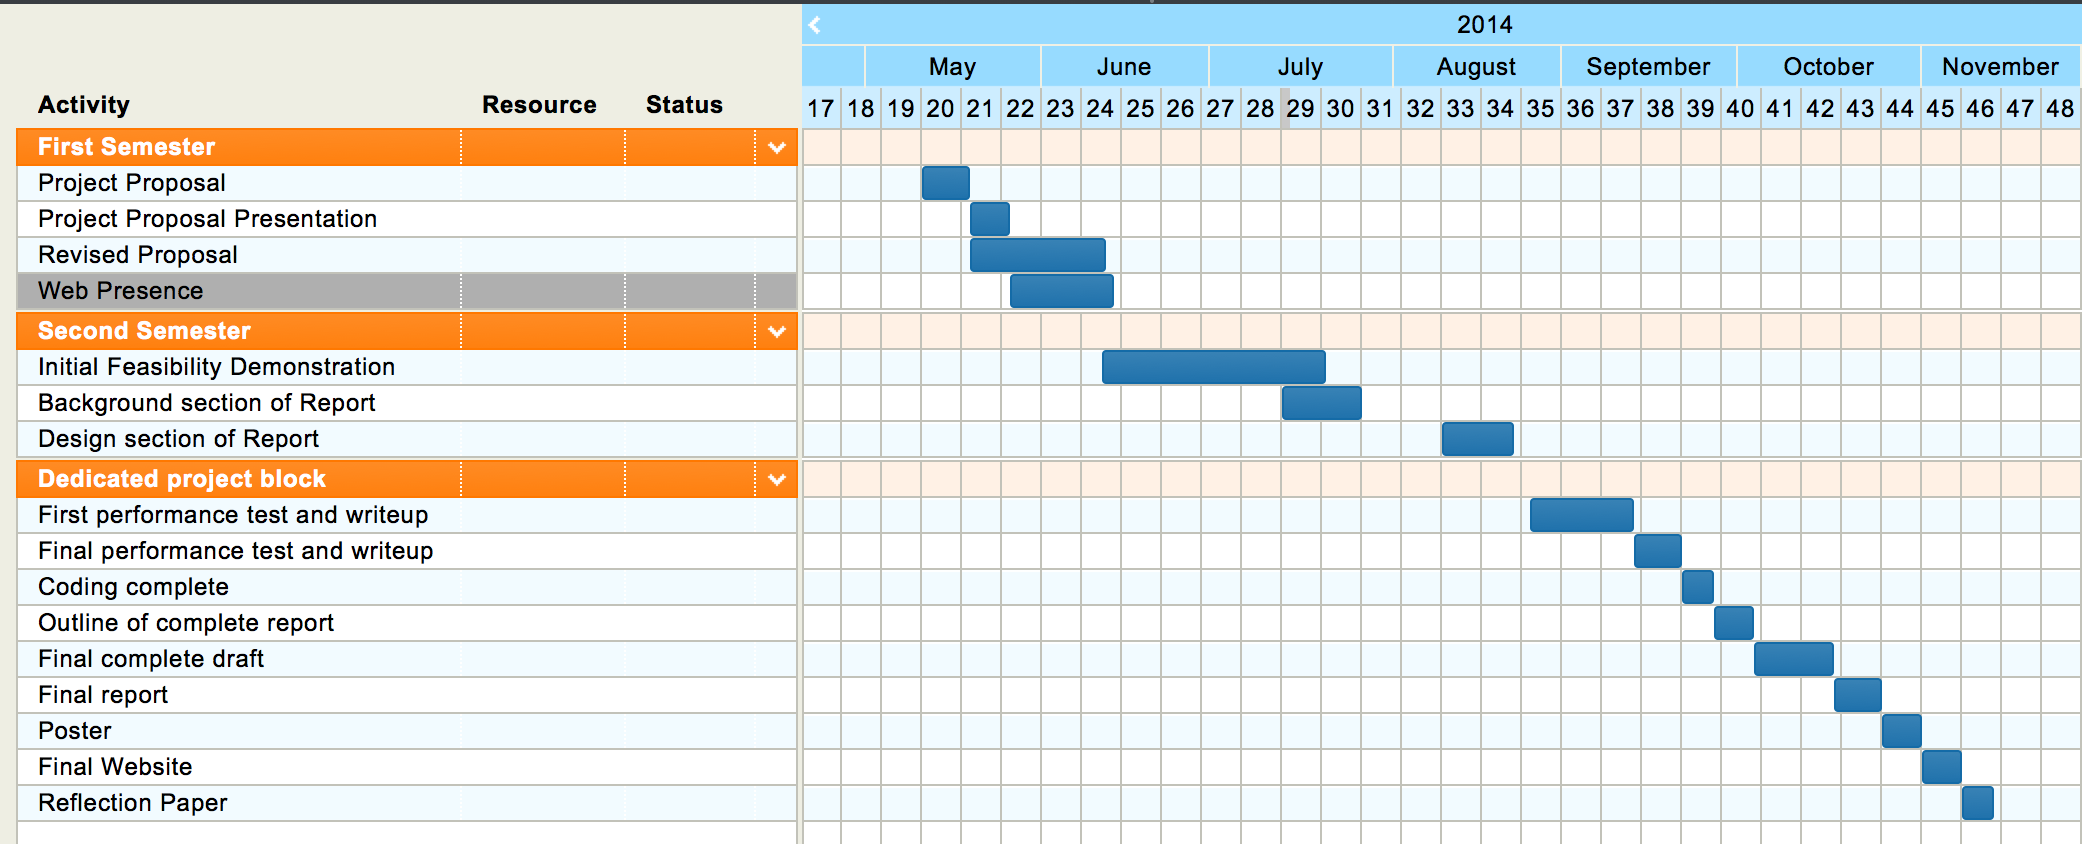
\includegraphics[scale=.4]{gantt}

The following resources will be required:

\begin{itemize}
    \item 
        \textbf{Generated data cubes
}

        These will be used to test the reliability and completeness of the CUDA implementations and to compare output with the original package.
    \item
        \textbf{Access to the GPU cluster}

        The GPU cluster at UCT is necessary to process large data cubes without blocking local use of personal computers and mitigate the effects of power outages.
    \item
        \textbf{HIPASS Parkes All Sky Survey data cubes as well as the catalogues for testing on 
real data and comparing reliability}

        HIPASS survey data cubes are required to test the performance of our accelerated source finder on real data in addition to generated data.
    \item
        \textbf{DUCHAMP and SoFiA source code}

        The CUDA implementations will be based on code in the DUCHAMP and SoFiA packages and integrated back into their respective repositories.
    \item
        \textbf{Workstations with CUDA enabled devices}

        CUDA runs on a range of NVIDIA graphics cards and it is a necessity to be able to run the implementations on a workstation with a CUDA enabled device.
\end{itemize}

A final report will be provided illustrating the comparison of the CUDA implementations overall processing time to that of the original package. These will be taken with respect to datacubes of varying sizes. An accompanying project poster and website will also be provided.

The following milestones relate to the sequence of work required to implement the CUDA version into the package. The higher level honors project milestones are provided in a gantt chart.


\begin{enumerate}
   \item Check out and build the package source code. We will have the source code checked out locally and in a buildable state. This is necessary in order to run the package with input.
   \item Obtain FITS datacube and run it through the package. This will be the first time the package has been run with input and produce output. We will need to understand the input parameters of the package in order to do so.
   \item Implement a single threaded version of our algorithm in C. This will require careful consideration into how the algorithm will be integrated and used by the package, and we will strive for minimal friction and maximal transparency to the user.
   \item Run performance tests with the single threaded implementation. These will be used as a base benchmark for the CUDA implementation.
   \item Naive GPU implementation. Have implemented a running, straightforward CUDA kernel, aiming for correctness and simplicity.
   \item Run performance tests on the naive GPU implementation. Use Nvidia’s profiling tools to analyse the CUDA implementation and gain insight to further optimise the CUDA kernel.
   \item Optimised GPU implementation. Have found grid sizes that maximise occupancy levels; local variables, data representation and use of memory hierarchies for optimal memory access times; and overlapping kernel execution to maximise on data transfer.
   \item Run performance tests on the optimised GPU implementation, to measure and profile the speedups over the naive implementation. We will likely iterate multiple times between this stage and the previous stage.
   \item Generate graphs to illustrate the running times of the optimised GPU implementation compared with the original package, over varying datacube sizes.
   \item Integrate code back into the package’s original source code repositories, or have approached the packages owners with permission to do so.
\end{enumerate}

Work has been divided into two independent projects designed to run in parallel with minimal dependencies. This mitigates the risk of a member dropping their project and allows the second project to continue unhampered. The two are essentially identical but each extends a different source code repository and attempts to accelerate aspects of different source finding algorithms. Each can read the same input data cubes, generate the same output and analyse the performance independently from the other.


Yaseen will accelerate 2D-1D wavelet reconstruction using CUDA and contribute towards the DUCHAMP package, released under GPLv3. Jarred will accelerate the S+C source finder using CUDA and contribute towards the SoFiA package, released under GPLv2.


Fig1 illustrates the work division between both Yaseen and Jarred, and indicates the stages that each will undergo. The stages are almost identical yet highly independent between the two projects.

\begin{figure}
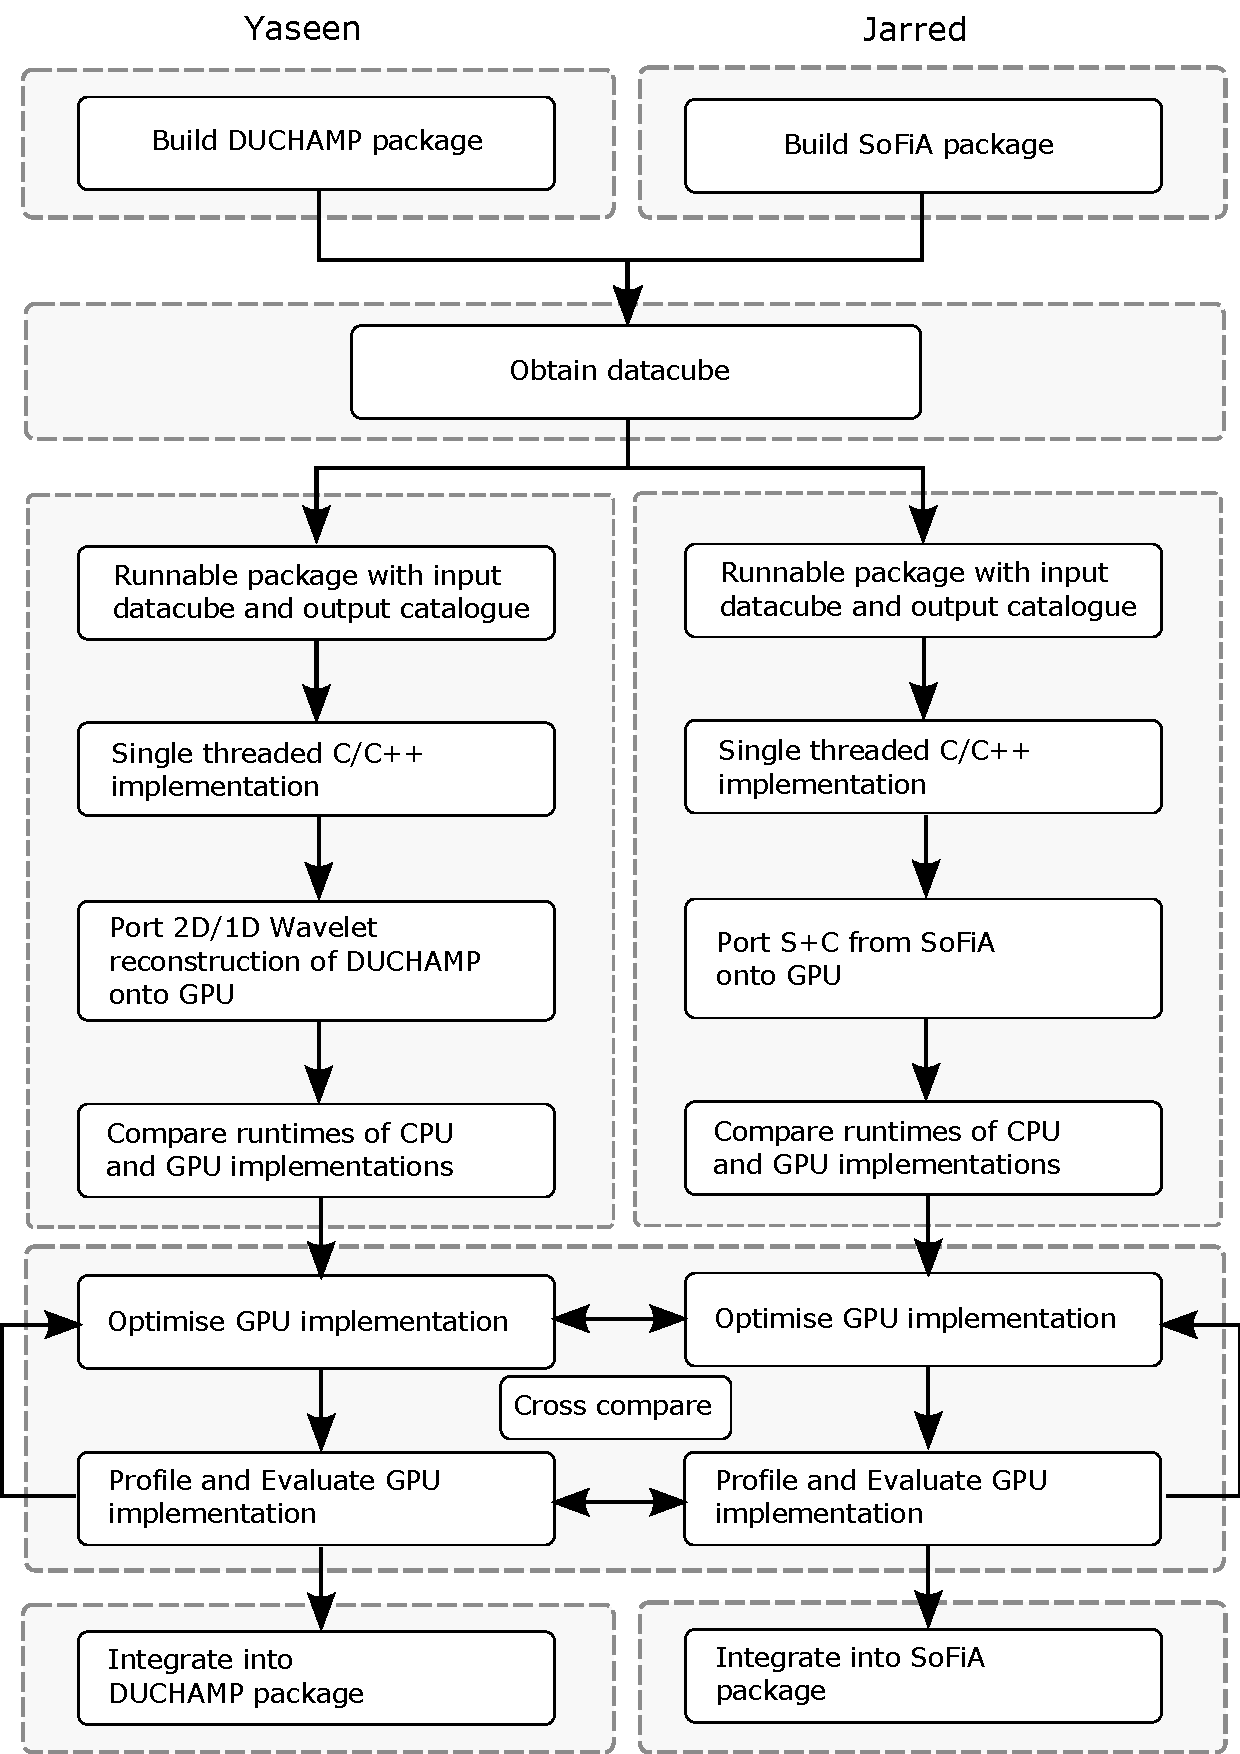
\includegraphics[scale=.65]{dependencies}
\caption{Work division between Yaseen and Jarred}
\end{figure}

\bibliographystyle{ACM-Reference-Format-Journals}
\bibliography{scaffold}

\end{document}
